% Created 2021-09-11 Sat 08:17
% Intended LaTeX compiler: xelatex
\documentclass[letterpaper]{article}
\usepackage{graphicx}
\usepackage{grffile}
\usepackage{longtable}
\usepackage{wrapfig}
\usepackage{rotating}
\usepackage[normalem]{ulem}
\usepackage{amsmath}
\usepackage{textcomp}
\usepackage{amssymb}
\usepackage{capt-of}
\usepackage{hyperref}
\usepackage[margin=1in]{geometry}
\usepackage{fontspec}
\usepackage{indentfirst}
\setmainfont[ItalicFont = LiberationSans-Italic, BoldFont = LiberationSans-Bold, BoldItalicFont = LiberationSans-BoldItalic]{LiberationSans}
\newfontfamily\NHLight[ItalicFont = LiberationSansNarrow-Italic, BoldFont       = LiberationSansNarrow-Bold, BoldItalicFont = LiberationSansNarrow-BoldItalic]{LiberationSansNarrow}
\newcommand\textrmlf[1]{{\NHLight#1}}
\newcommand\textitlf[1]{{\NHLight\itshape#1}}
\let\textbflf\textrm
\newcommand\textulf[1]{{\NHLight\bfseries#1}}
\newcommand\textuitlf[1]{{\NHLight\bfseries\itshape#1}}
\usepackage{fancyhdr}
\pagestyle{fancy}
\usepackage{titlesec}
\usepackage{titling}
\makeatletter
\lhead{\textbf{\@title}}
\makeatother
\rhead{\textrmlf{Compiled} \today}
\lfoot{\theauthor\ \textbullet \ \textbf{2021-2022}}
\cfoot{}
\rfoot{\textrmlf{Page} \thepage}
\titleformat{\section} {\Large} {\textrmlf{\thesection} {|}} {0.3em} {\textbf}
\titleformat{\subsection} {\large} {\textrmlf{\thesubsection} {|}} {0.2em} {\textbf}
\titleformat{\subsubsection} {\large} {\textrmlf{\thesubsubsection} {|}} {0.1em} {\textbf}
\setlength{\parskip}{0.45em}
\renewcommand\maketitle{}
\author{Houjun Liu}
\date{\today}
\title{The Lifecycle of a Cell}
\hypersetup{
 pdfauthor={Houjun Liu},
 pdftitle={The Lifecycle of a Cell},
 pdfkeywords={},
 pdfsubject={},
 pdfcreator={Emacs 27.2 (Org mode 9.4.4)}, 
 pdflang={English}}
\begin{document}

\maketitle


\section{The Cell('s) (Life)Cycle}
\label{sec:orgfc254b5}
\subsection{So, why do cell divide}
\label{sec:orgcd00d68}
Everyday, 50-70 Billion die (\textbf{programmed cell death}, apoptosis), so\ldots{}

\begin{quote}
The ability to produce organisms more of their kind is one
characteristic that best distinguishes living things from nonliving
matter
\end{quote}

\href{KBhBIO101Viruses.org}{KBhBIO101Viruses} and organelles challenge
this definition => they are symbiotic and cannot reproduce on their own.
But like screw them right?

To compensate for programmed cell death, (cell division) happen.

\textbf{Before we continue, do yourself a favor and review
\href{KBhBIO101DNAStructures.org}{KBhBIO101DNAStructures}}

\subsection{So, when do cells divide? (The Actual Cell Cycle)}
\label{sec:org50fd3d5}
The cell follows a lifecycle from new cell to
cell-too-bit-aaa-gotta-divide called\ldots{} you ready for this? "Cell
Cycle". At the pointy bit of the cell cycle, the cell reproduces
\href{KBhBIO101CellReproduction.org}{KBhBIO101CellReproduction}. And
et viola the cell cycle!

For more, see \href{KBhBIO101CellCycle.org}{KBhBIO101CellCycle}.

\begin{figure}[htbp]
\centering
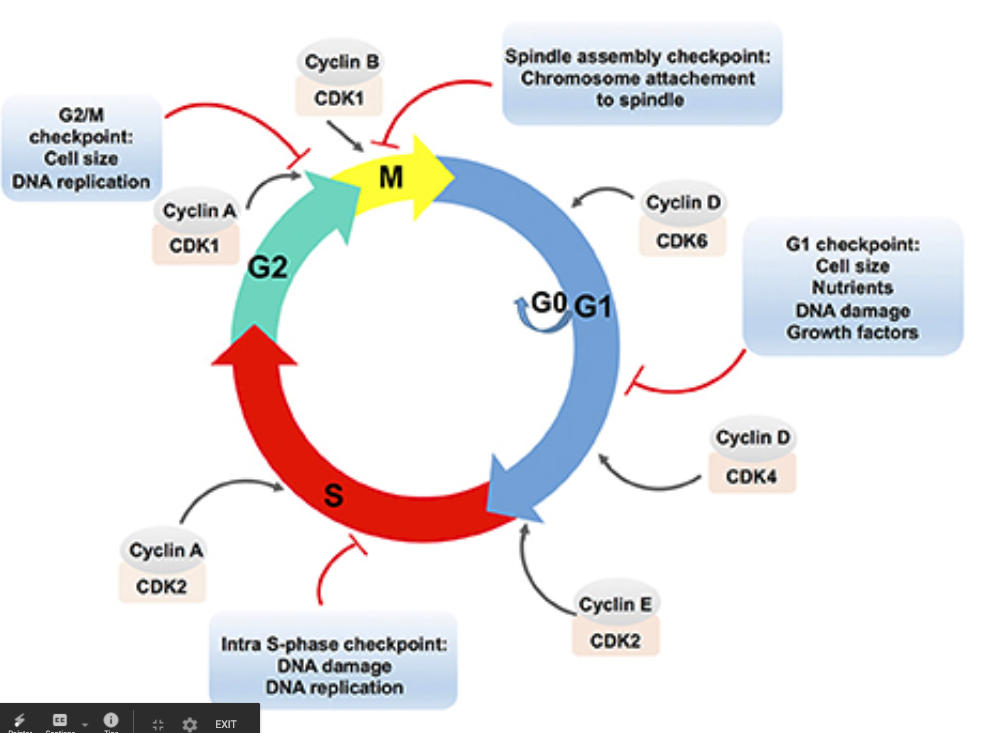
\includegraphics[width=.9\linewidth]{lecellcycle.png}
\caption{lecellcycle.png}
\end{figure}

\subsection{So, how do cells divide?}
\label{sec:org572f83f}
\href{KBhBIO101CellReproduction.org}{KBhBIO101CellReproduction}
\end{document}
